% --- Program Section ---

\newprogram{Program 4}{Implement strassen-multiply(A: List[List[int]], B: List[List[int]]) ->
List[List[int]] accepting two matrices and returning their product matrix.}

\subsection*{Code}
\begin{lstlisting}[language=Python]
from typing import List

def strassen_multiply(A: List[List[int]], B: List[List[int]]) -> List[List[int]]:
    n = len(A)

    # Base case
    if n == 1:
        return [[A[0][0] * B[0][0]]]

    # Split matrices into 4 parts
    mid = n // 2

    A11 = [row[:mid] for row in A[:mid]]
    A12 = [row[mid:] for row in A[:mid]]
    A21 = [row[:mid] for row in A[mid:]]
    A22 = [row[mid:] for row in A[mid:]]

    B11 = [row[:mid] for row in B[:mid]]
    B12 = [row[mid:] for row in B[:mid]]
    B21 = [row[:mid] for row in B[mid:]]
    B22 = [row[mid:] for row in B[mid:]]

    def add(X, Y):
        return [[X[i][j] + Y[i][j] for j in range(len(X))]
                for i in range(len(X))]

    def subtract(X, Y):
        return [[X[i][j] - Y[i][j] for j in range(len(X))]
                for i in range(len(X))]

    # Strassen's 7 multiplications
    M1 = strassen_multiply(add(A11, A22), add(B11, B22))
    M2 = strassen_multiply(add(A21, A22), B11)
    M3 = strassen_multiply(A11, subtract(B12, B22))
    M4 = strassen_multiply(A22, subtract(B21, B11))
    M5 = strassen_multiply(add(A11, A12), B22)
    M6 = strassen_multiply(subtract(A21, A11), add(B11, B12))
    M7 = strassen_multiply(subtract(A12, A22), add(B21, B22))

    # Calculate result quadrants
    C11 = add(subtract(add(M1, M4), M5), M7)
    C12 = add(M3, M5)
    C21 = add(M2, M4)
    C22 = add(subtract(add(M1, M3), M2), M6)

    # Combine quadrants
    result = []

    for i in range(mid):
        result.append(C11[i] + C12[i])

    for i in range(mid):
        result.append(C21[i] + C22[i])

    return result


# Example
A = [
    [1, 2],
    [3, 4]
]

B = [
    [5, 6],
    [7, 8]
]

print(strassen_multiply(A, B))
\end{lstlisting}

\subsection*{Output}
\begin{center}
    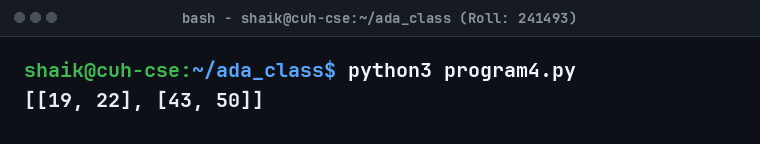
\includegraphics[width=0.88\textwidth]{Images/output_screenshot4.png}
\end{center}

\subsection*{GitHub Scan Code}
\begin{center}
    \begin{minipage}{0.3\textwidth}
        \centering
        % Generates a 2.5cm high QR code directly linking to the code file
        \qrcode[height=3.5cm]{https://github.com/gytdrop/ada_class/blob/main/program4.py} \\[0.2cm]
        \scriptsize\ttfamily Scan to view source code 
    \end{minipage}
\end{center}


% Add a horizontal line that indicates the END of the program.
\vspace{1cm}
\begin{center}
    \rule{1\textwidth}{1pt} % Clean, centered 1pt thick horizontal line
\end{center}